\documentclass{article}

\usepackage{graphicx}
\usepackage{caption}
\usepackage{subcaption}
\usepackage{booktabs}
\usepackage{csvsimple}
\usepackage{amsmath}
\usepackage{listings}
\usepackage{url}
\usepackage{mwe}

\usepackage{amsopn}
\DeclareMathOperator{\cov}{cov}
\DeclareMathOperator{\var}{var}

\lstset{inputpath=../algo/R_final}
\usepackage[style=authoryear,backend=biber]{biblatex}
% Set library for biblatex
\bibliography{library}

\usepackage{tikz}
\usetikzlibrary{bayesnet}
\usetikzlibrary{positioning}

\title{Predicting positions using Independence Graphs}
\author{Volker Strobel}
\date{\today}

\graphicspath{{img/}}

\begin{document}
\maketitle

% Inducing Features of Random Fields (Pietra)

% I can start with one feature and
% successively include more and more features, until my prediction
% becomes better and better.

% Test on hold-out test see

% Archimedean copulas are an associative class of copulas. Most common
% Archimedean copulas admit an explicit formula, something not
% possible for instance for the Gaussian copula. In practice,
% Archimedean copulas are popular because they allow modeling
% dependence in arbitrarily high dimensions with only one parameter,
% governing the strength of dependence

% Linear regression

% Greedy approach for feature inclusion

% MSE minimizes the expected error
% Another error function minimizes the model

% http://www.r-bloggers.com/modelling-dependence-with-copulas-in-r/

\begin{abstract}
  In this report, the dependence structure between image features and
  $x,y$-coordinates is analyzed using linear regression, graphical
  Gaussian models, and vine copulas. The dependencies between average
  color per channel and image location are used to build a predictive
  model for given image features. The predictive power of the used
  models are compared using the mean absolute error of the predictions
  on a hold-out test set. The associated uncertainty in the
  predictions are studied and indications are given, how the proposed
  model can be used in a real-world scenario.
\end{abstract}


\section{Introduction \& Problem Statement}

% This could be used in the context of a UAV flight...

% The report will use the notation of \cite{whittaker2009graphical}.


% Idea: use red as an indicator of the environment and add x,y,env as
% prediction goal.

Computer vision tasks---such as object detection, image restoration,
or \emph{localization}---often need a high-dimensional reprentation of
a feature domain. This task can be fulfilled using probabilistic
graphical models and has been used in a variety of applications.

Combining copula modelling with machine learning techniques was
longtime neglected---and to date, many problems are studied in the
bivariate case only. However, recently, more and more research is
focusing on combining machine learning and regression techniques to
tackle high-dimensional regression problems
\parencite{cooke2015vine,elidan2013copulas}.

In this report, we consider the following computer vision localization
problem:
\begin{quote}
  Based on a given patch of an image, we would like to predict, where
  the patch was taken in a larger image---the map image.
\end{quote}
While existing approaches extract keypoints of the current patch and
the map image, followed by finding a homography between both keypoint
sets, these approaches are usually computationally complex and do not
allow for in-depth analyses of the problem (e.g. how to change the map
image to improve the quality of the algorithm).

This report addresses this multivariate problem consisting of five
random variables: average red, green, and blue value of an image patch
and corresponding $x, y$-position of the patch in a larger map
image. The dataset has been obtained by generating random image
patches from a given map image. These image patches could simulate
camera images obtained during a flight with a micro aerial vehicle
(MAV) over the map image.

% The problem is addressed based on two approaches: (i) modifying the
% environment (i.e., the map image) to make it better suited for the
% used approach, and (ii) modify the approach to make it better suited
% to the given map image.

The goal of this report is to compare models for predicting the
$x,y$-coordinate of unseen image patches. To this end, dependency
models are infered that are able to capture the multivariate
distribution of the sample data. We compare approaches using linear
regression, graphical Gaussian models, and vine copulas.

The use of \emph{copulas} allows to model marginal
distributions and dependence structure independently, allowing for
convenient and powerful representation of joint probability
distributions. Vine copulas leverage these advantages and bring the
advantages to higher dimensional distributions.

The vine copula approach is based on Sklar's theorem that states that
multivariate distribution can be described by marginal distributions
and the dependence structure---the copulas. Using bivariate copulas as
building blocks, more complex interaction structures can be achieved
by building \emph{vine copulas}---nested sets of connected trees.

% Therefore, we address the same problem from three viewing angles.

The remainder of this report is structured as
follows. Section~\ref{sec:methods} introduces the method for
generating the dataset, and for inferring the linear least square
predictor, graphical Gaussian models, and vine
copulas. Section~\ref{sec:results} shows the obtained results with
respect to root mean squared error (RMSE). In
Section~\ref{sec:discussion}, the results are discussed and models are
compared. Finally, in Section~\ref{sec:conclusion}, conclusions and
future research directions are given.

\section{Methods}
\label{sec:methods}

\subsection{Dataset Generation}

For generating a dataset, a suitable map image was chosen. Since the
color distribution should be related to the position of the image
patch---and not randomly spread over the image---the search term
'rainbow art' was used in Google's image search. Rainbow art features
an image gradient, without having a too strong or too weak correlation
between mean color and $x, y$ position. The selected image can be seen
in Figure~\ref{fig:generation}.

In order to obtain image patches from a given map image, $N=1000$
different views of the map image are generated using the tool
\emph{draug}\footnote{draug is a tool that I developed during my
  graduation project. It can be found on:
  \url{https://github.com/Pold87/draug}}. The camera positions are
sampled from a normal distribution with the following parameters:
\begin{align}
  (x, y) &\sim \mathcal{N}(\mu, \Sigma)\\
  \mu &=
  \begin{pmatrix}
    0.5\\
    0.5\\
  \end{pmatrix}
\\
  \Sigma &= \begin{pmatrix} 107 & 0\\
    0 & 80 \end{pmatrix}
\end{align}
Therefore, $x$ and $y$ positions are sampled independently. The
standard deviations were chosen, such that 99\,\% of the data points
are expected to be in the ranges $[0, 640]$ and $[0, 480]$,
respectively for $x$, and $y$ values. The resulting dataset can be
found in the appendix. 500 of the images are used as training images
and 500 as test images.

% Due to the simulation, the availability of the data is not a problem
% and new data can be easily generated. The presented approach is
% largely data-driven but also exploits the knowledge of the
% construction of the dataset.

% Figure~\ref{fig:generation} shows the process of data set
% generation. To this end, we will construct a generative model
% $p(x,y,R,G,B)$ for the distribution. We decided to create the
% generative model, since it allows to construct an image from the
% trained model.

% In the case of the graphical models, the regression will be
% performed by deriving a point estimate (mean, median, mode) from the
% distribution $p(x,y \mid R,G,B)$.

% Since we will deal with Gaussian distributions, the three point
% estimates fall together.

\begin{figure}
  \centering
  \begin{subfigure}[b]{0.4\textwidth}
    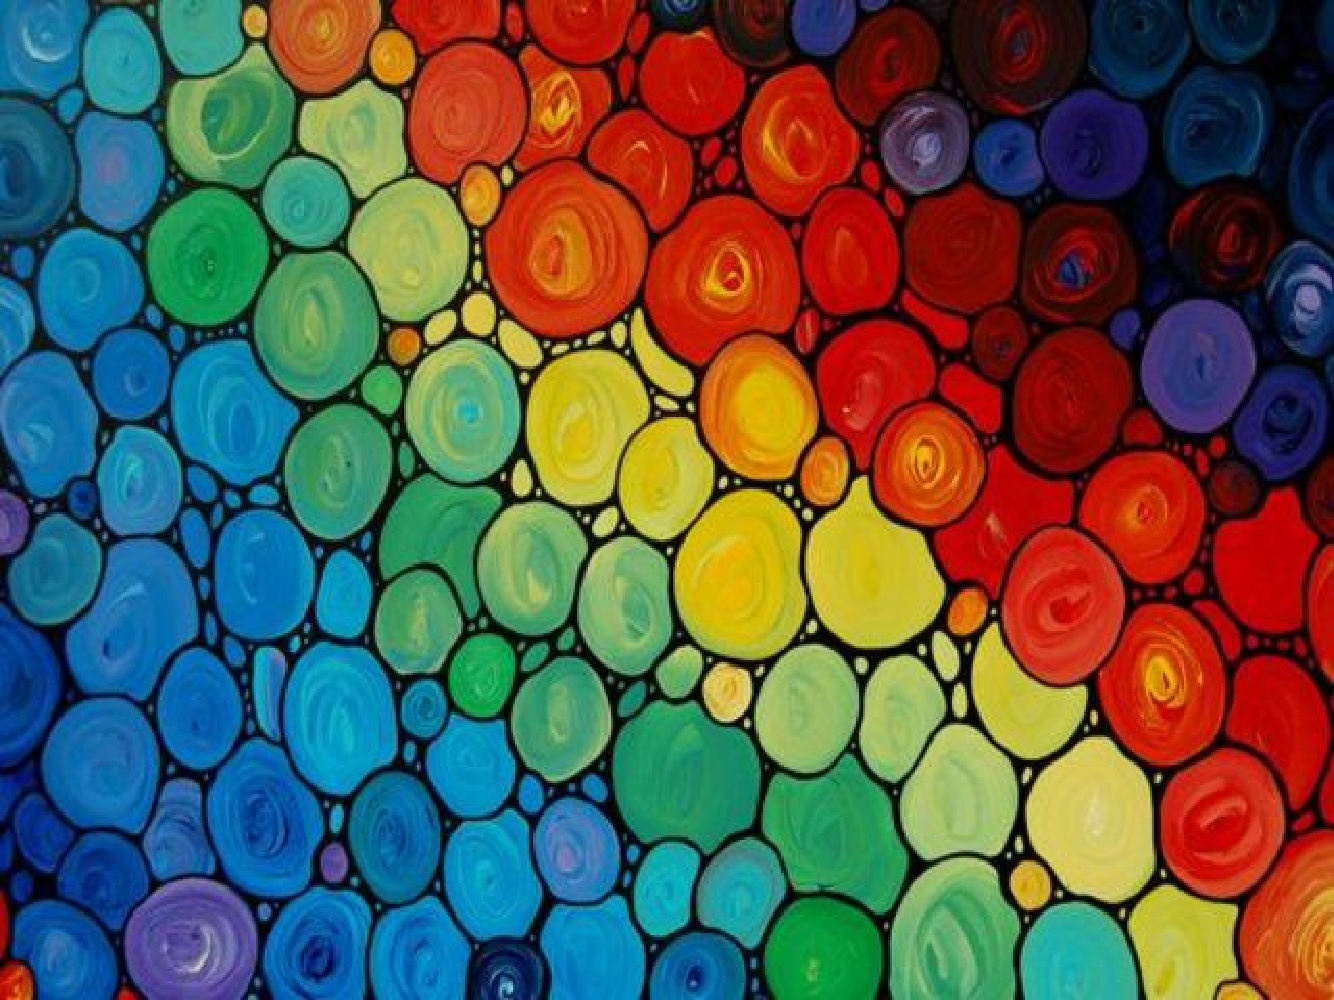
\includegraphics[width=\textwidth]{rainbow}
    \captionof{figure}{Map image}
    \label{fig:mapimage}
  \end{subfigure}%
~
  \begin{subfigure}[b]{0.4\textwidth}
    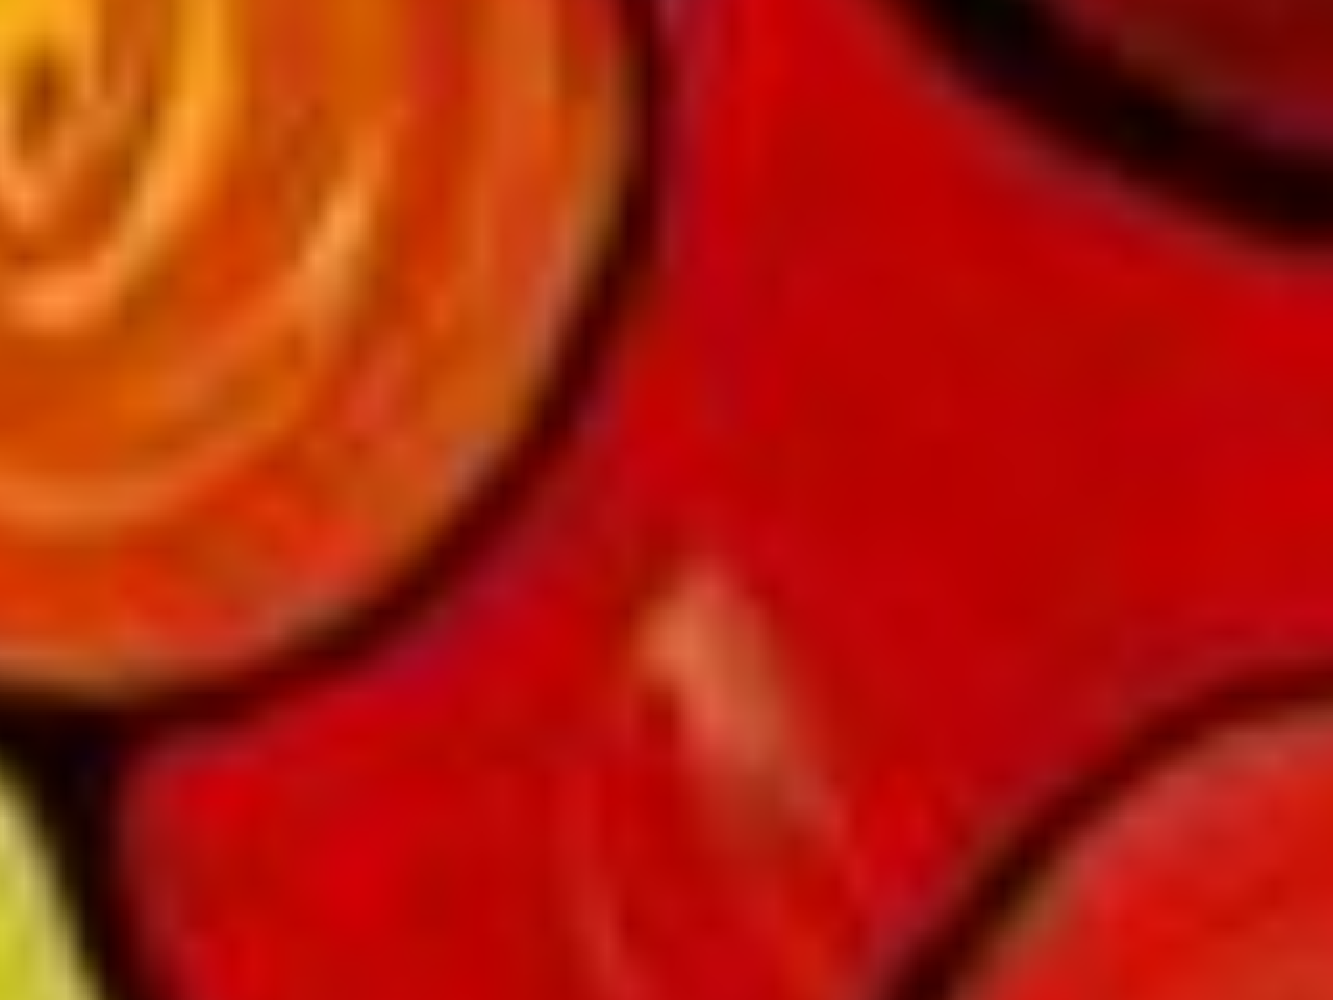
\includegraphics[width=\textwidth]{patch}
    \captionof{figure}{Random image patch}
    \label{fig:patch}
  \end{subfigure}
  \caption{Figure~\ref{fig:mapimage} Shows the map image that is used
    for generating the image patches. Figure~\ref{fig:patch} shows one
    sample of the $N = 1000$ image patches that were generated for the
  generation of the data set.}
\label{fig:generation}
\end{figure}

Three features per image patch are used: the average red, green, and
blue color. The data set based on $N = 1000$ image patches can be
found in the appendix. By construction of the dataset, it is known
that the samples are identically and independently distributed
(i.i.d).

\subsection{Test for Normality}

For motivating the use of graphical Gaussian models, the Shapiro-Wilk
test is used (significance level $\alpha = 0.05$), which tests if the
univariate marginal distributions are normally distributed.

\subsection{Linear Least Squares Predictor}
\label{sec:llsp}

% TODO: x and y are used for positions. This is confusing, especially
% the smaller letters.

The used random vectors are $Y = (x, y)$ and $X = (R, G, B)$. Given a
measurement of the average color values $X = \textbf{x} = (r, g, b)$,
the linear least squares predictor is calculated as follows:
\begin{align*}
  \hat{Y}(X) & = EY + \cov(Y, X)\var(X)^{-1}(\textbf{x}-EX) \\
\end{align*}
The explained variation $R^2$ and residual variance are calculated.


\subsection{Gaussian Graphical Model}

A Gaussian graphical model from the training set is constructed. Two
steps are involved in this procedure: model selection, that is, the
construction of the independence graph and likelihood inference for
the variance matrix $V$.
% The graph is constructed using the $\chi^2$
%test for independence and the variance matrix is fit using iterative
%proportional fitting (IPF).
Log-likelihood and deviance compared to the saturated model are
calculated.

% The following conditional independence statements can be read from
% the graph.

\subsubsection{Model Selection}

% While a thresholded exclusions strategy (e.g. corr $<$ 0.1) seems
% directly accessible, it does not capture the size and therefore
% available information of the sample data.

For selecting the model, sequential backward elimination from a
saturated graphical model is used. In each step, the edge with the
highest $p$-value based on the $\chi^2$ test of independence is
deleted. If no $p$-value is significant (significance level
$\alpha=0.05$), the iteration is stopped.\\

\subsubsection{Fitting}

Based on the graphical model achieved in the model selection step, the
maximum likelihood estimate of the variance matrix $V$ is calculated
using the the IPF algorithm. The IPF algorithm updates the sample
variance matrix and fits it to the given graph. 


\subsubsection{Predictions}

The expectation $E_{b | a}(X_b)$ is used to calculate the point
estimate.  Using Proposition 6.3.1 \parencite{whittaker2009graphical},
the conditional distribution of $X_b$ given $X_a = a$ is normally
distributed with mean
\begin{align}
  E_{b | a}(X_b) = \mu_b + V_{ba}V^{-1}_{aa}(x_a - \mu_a)
\end{align}
and variance
\begin{align}
  \text{var}_{b|a}(X_b) = V_{bb|a} = V_{bb} - V_{ba}V_{aa}^{-1}V_{ab}
\end{align}
R, G, B are given, while $x,y$ are desired. Therefore, $X_a = (R, G,
B)$ and $X_b = (x,y)$. The equation for $E_{b | a}(X_b)$ directly
related to the linear least squares predictor using the fitted matrix
$V$, where $V_{ba}$ relates to $\cov(Y, X)$ and $V^{-1}_{aa}$ to
$\var(X)^{-1}$.

% $\mu_b = (320, 240)$ is the center point of the image.

%As expected, the conditional mean and the linear least square
%predictor are identical (see Corollary 6.3.2).The higher variance in
%the x coordinate of the conditional distribution is directly related
%to the $R^2$ value.

\subsection{Vine Copula}

Finally, the dependence structure between the variables is described
using vine copulas. The samples are converted to pseudo observations
and ties are broken at random. The tree structure of the vine is
chosen using forward selection. The selection is performed among all
possible families in the R package \emph{Vine Copula}\footnote{An
  overview of the possible families can be found at:
  \url{https://cran.r-project.org/web/packages/VineCopula/VineCopula.pdf}}. To
this end, the available copulas are fitted using maximum likelihood
estimation. Then, bivariate copula families for the edges of the vine
are chosen using log-likelihood as selection criterion.

% While it is theoretically possible to get $F(x)$ by evaluating it at
% \ldots, in practice we have to calculate the inversion of the
% (empiricial / pseudo) CDF.
                                          
\section{Results}
\label{sec:results}

\subsection{Test for Normality}

% TODO: see if copula package plot is better
Figure~\ref{fig:pairwise} shows the pairwise correlation plot of the
training dataset. It can be seen that the variables $R, G, B$ seem to
be non-normally distributed. This is underlined by Shapiro-Wilk's
Normality Test (Table~\ref{tab:shapiro}).
\begin{figure}[h]
  \centering
  \includegraphics[width=0.9\textwidth]{../algo/R_final/data}
  \caption{This figure shows a scattermatrix of the training
    dataset. The upper triangle displays the Spearman correlation
    coefficients (asterisks indicate significance level), the diagonal
    displays the histograms and kernel density estimates, and the
    lower diagonal shows the bivariate sample distributions.}
  \label{fig:pairwise}
\end{figure}
\begin{table}[h]
  \centering
  \begin{tabular}{llll}
    \toprule
    Variable & Statistic & $p$-value & Normality \\
    \midrule
    R        & 0.8941    & 0.0000  & no        \\
    G        & 0.8843    & 0.0000  & no        \\
    B        & 0.9183    & 0.0000  & no        \\
    x        & 0.9979    & 0.2373  & yes       \\
    y        & 0.9983    & 0.4175  & yes       \\
    \bottomrule
  \end{tabular}
  \caption{Shapiro-Wilk's normality test}
  \label{tab:shapiro}
\end{table}
Still, the analysis is continued assuming a multivariate normal
distribution.

\subsection{Linear least squares predictor}


% \begin{figure}[h]
%   \centering
%   \includegraphics[width=0.85\textwidth]{../algo/img/pairs_copuladata.pdf}
%   \caption{Analysis of pairs of copula data.}
%   \label{fig:pairscopula}
% \end{figure}

% Table created by stargazer v.5.2 by Marek Hlavac, Harvard University. E-mail: hlavac at fas.harvard.edu
% Date and time: Fri, Jun 17, 2016 - 04:48:42 PM
\begin{table}[h] \centering 
\begin{tabular}{l|rrrrr} 
R     & $0.05$  &          &          &          &         \\ 
G     & $-0.01$ & $0.04$  &          &          &         \\ 
B     & $-0.03$ & $0.02$  & $0.03$  &          &         \\ 
x     & $0.02$  & $-0.01$ & $-0.02$ & $0.03$  &         \\ 
y     & $-0.02$ & $0.01$  & $0.01$  & $0.00$ & $0.03$ \\ 
\midrule
means & $0.49$   & $0.43$   & $0.22$   & $0.50$   & $0.49$  \\
\midrule
      & R        & G        & B        & x        & y       \\ 
\end{tabular} 
\caption{The sample variance matrix of the data set. The variances are calculated  using the operator $\var_{500}(X,Y).$}
\label{tab:var}
\end{table} 

% \begin{table}[h]
% \  \centering
%   \begin{tabular}{l|rrrrr}
%     red   & 1.00  &       &       &      &      \\
%     green & 0.46  & 1.00  &       &      &      \\
%     blue  & 0.32  & 0.75  & 1.00  &      &      \\
%     x     & -0.13 & -0.05 & -0.04 & 1.00 &      \\
%     y     & -0.13 & -0.06 & 0.09  & 0.03 & 1.00 \\
%     \midrule
%           & red   & green & blue  & x    & y
%   \end{tabular}
%   \caption{The sample correlation matrix of the data set}
% \end{table}

% \begin{table}                                   
% \centering                                      
% \begin{tabular}{l|rrrrr}                    
%     red   & 1.30  &       &       &       &      \\  
%     green & -0.59 & 2.64  &       &       &      \\
%     blue  & 0.02  & -1.81 & 2.37  &       &      \\ 
%     x     & 0.14  & -0.02 & 0.01  & 1.02  &      \\ 
%     y     & 0.13  & 0.24  & -0.32 & -0.01 & 1.06 \\ 
%   \midrule
%   $R^2$   & 0.23  & 0.62  & 0.58  & 0.02  & 0.06 \\
%   \midrule
%           & red   & green & blue  & x     & y
% \end{tabular}                                   
% \caption{Inverse correlation matrix}                        
% \label{table:MyTableLabel}                      
% \end{table} 

Table~\ref{tab:var} shows the empirical variance matrix and the mean
values of the training dataset.  Given a measurement of the average
color values $X = \textbf{x} = (r, g, b)$, the linear least squares
predictor becomes:
\begin{align*}
  \hat{Y}(X) & = EY + \cov(Y, X)\var(X)^{-1}(\textbf{x}-EX) \\
  & =
          \begin{pmatrix}
            0.50\\
            0.49
          \end{pmatrix} +
  \begin{pmatrix}
    0.02  & -0.01 & -0.02                      \\
    -0.02 & 0.01  & 0.01                       \\
  \end{pmatrix}
  \begin{pmatrix}
    0.05 & -0.01 & -0.03\\
    -0.01 & 0.04 & 0.02\\
    -0.03 & 0.02 & 0.03\\
  \end{pmatrix}^{-1}
  \begin{pmatrix}
    r - 0.49\\
    g - 0.43\\
    b - 0.22\\
  \end{pmatrix}\\
& =
\begin{pmatrix}
  0.68 + 0.01r - 0.11g - 0.64b\\
  0.60 - 0.45r + 0.36g - 0.15b\\
\end{pmatrix}
\end{align*}
\begin{table}[h] \centering 
\begin{tabular}{l|rrrrr} 
R & $7.02$  &         &         &         &        \\ 
G & $-3.46$ & $3.30$  &         &         &        \\ 
B & $5.47$  & $-2.55$ & $8.95$  &         &        \\ 
x & $-1.57$ & $1.59$  & $2.08$  & $4.00$  &        \\ 
y & $1.97$  & $-1.68$ & $-1.02$ & $-2.49$ & $3.20$ \\ 
\midrule
  & R       & G       & B       & x       & y      \\ 
\end{tabular} 
\caption{Inverse correlation matrix}
\label{tab:invcor}
\end{table} 
In Table~\ref{tab:invcor}, the inverse correlation matrix is
shown. From the table, the proportion of explained variation for $x$
and $y$ can be calulated:
\begin{align*}
  R^2(x; rest) &= (4.00 - 1) / 4.00 = 75\,\%\\
  R^2(y; rest) &= (3.20 - 1) / 3.20 = 68.75\,\%\\
\end{align*}
% Table created by stargazer v.5.2 by Marek Hlavac, Harvard University. E-mail: hlavac at fas.harvard.edu
% Date and time: Fri, Jun 17, 2016 - 08:20:42 PM
% TODO: include accounted variance, residual variance and prediction
% interval
The determined coefficients from Section~\ref{sec:methods} are used to
obtain $x, y$-predictions for the $N = 500$ test images. A root mean
squared error (RMSE) of 0.13 and 0.15 has been obtained for the $x$
and $y$ coordinate, respectively.

% \begin{figure}
%   \centering
%   \begin{subfigure}[b]{0.5\textwidth}
%     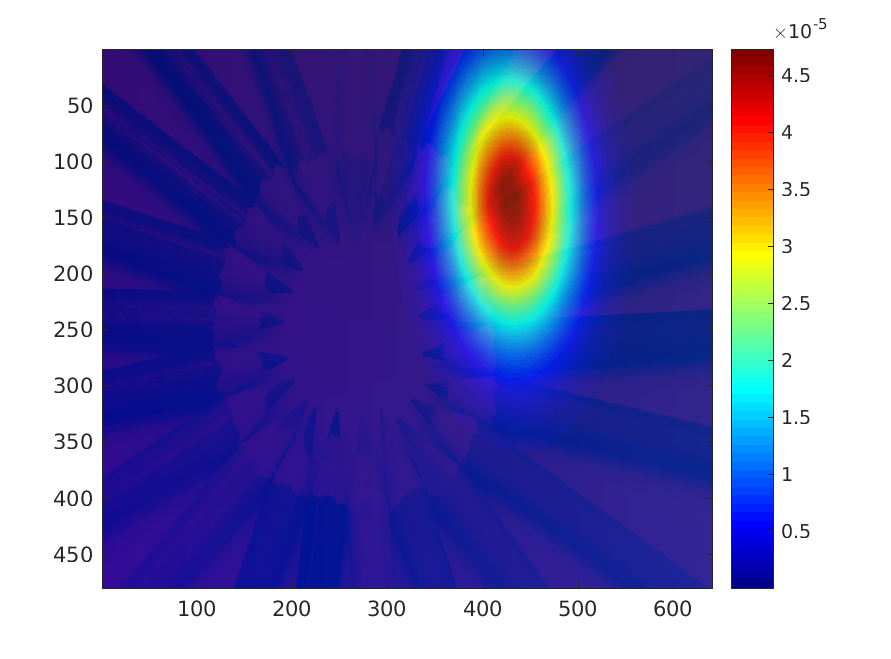
\includegraphics[width=\textwidth]{dorota_img.pdf}
%     \captionof{figure}{Graphical representation of the vine.}
%     \label{fig:heatmap}
%   \end{subfigure}%
% ~
%   \begin{subfigure}[b]{0.45\textwidth}
%     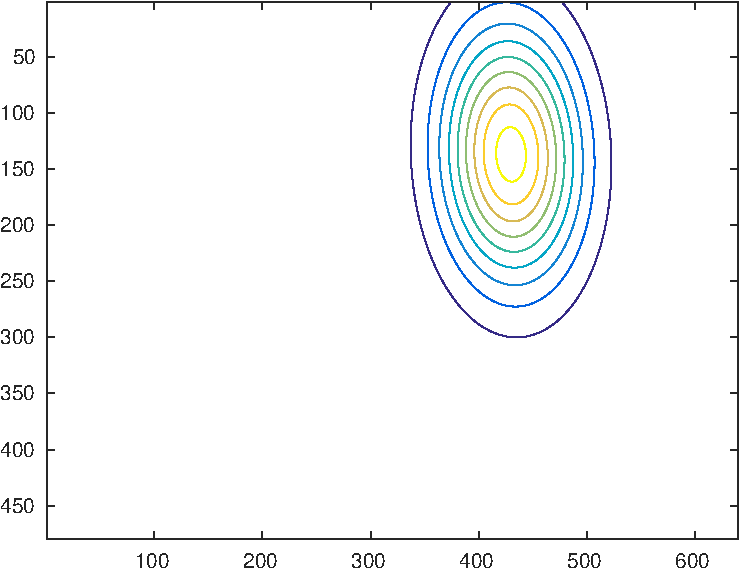
\includegraphics[width=\textwidth]{dorota_contour-crop}
%     \captionof{figure}{Contour plot}
%     \label{fig:contour}
%   \end{subfigure}
%   \caption{The density of the contour plot is density is coupled with
%     standard normal margins.}
% \label{fig:predvisualization}
% \end{figure}


% \begin{figure}
%   \centering
%   \begin{subfigure}[b]{0.5\textwidth}
%     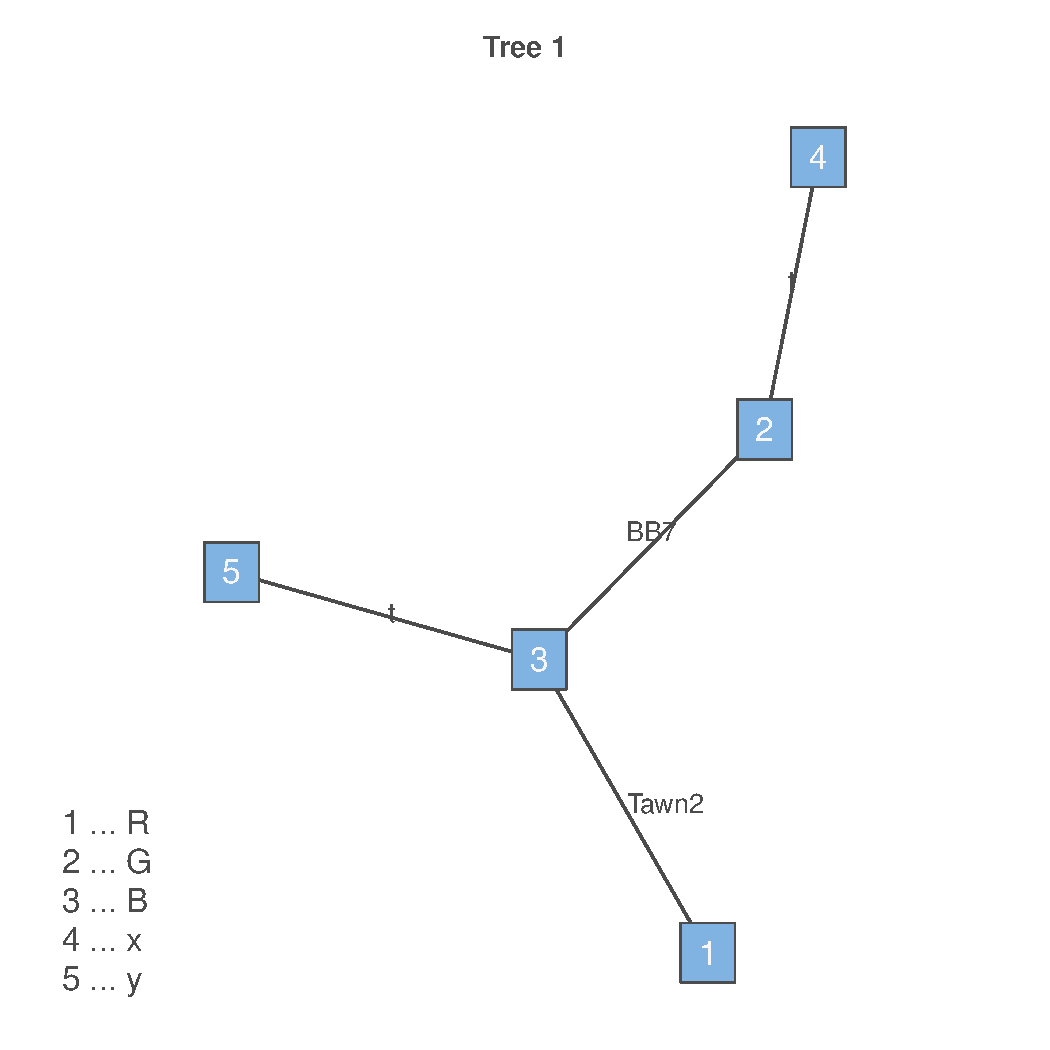
\includegraphics[width=\textwidth]{tree1}
%     \captionof{figure}{Image overlay}
%     \label{fig:heatmap}
%   \end{subfigure}%
% ~
%   \begin{subfigure}[b]{0.45\textwidth}
%     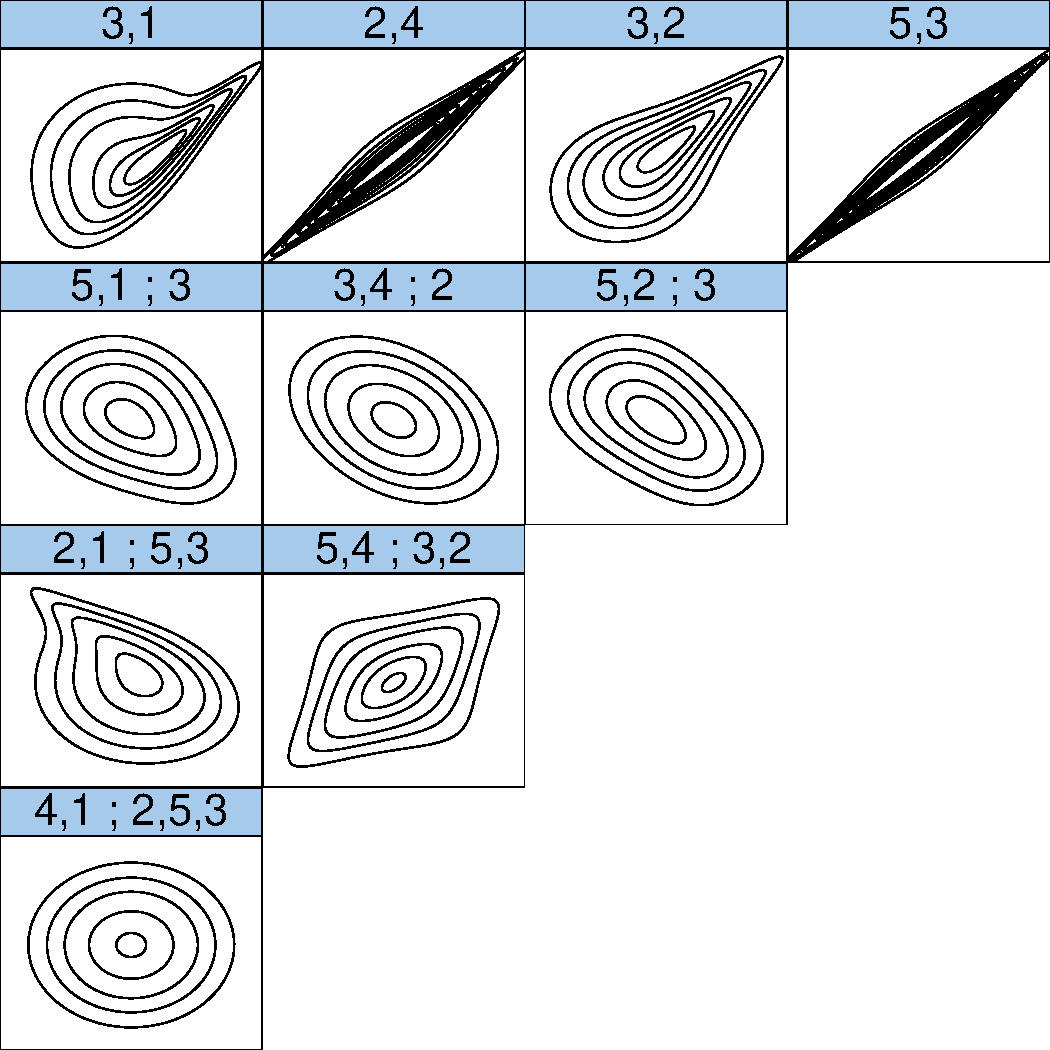
\includegraphics[width=\textwidth]{contour_copula}
%     \captionof{figure}{Contour plot}
%     \label{fig:contour}
%   \end{subfigure}
%   \caption{Example of the visualization of the predictions using RGB =
%     (100, 70, 200)}
% \label{fig:predvisualization}
% \end{figure}

\subsection{Gaussian Graphical Model}

In the first iteration of the backward elimination method, the edge
$\{x, y\}$ is deleted ($\chi^2=0.0013, p = 0.972$). In the second
iteration, the edge $\{G, x\}$ is deleted ($\chi^2=1.165, p =
0.281$). This process yields the graphical model in
Figure~\ref{fig:ggm}.

% TODO: deviance etc.

\begin{figure}[h]
  \centering
  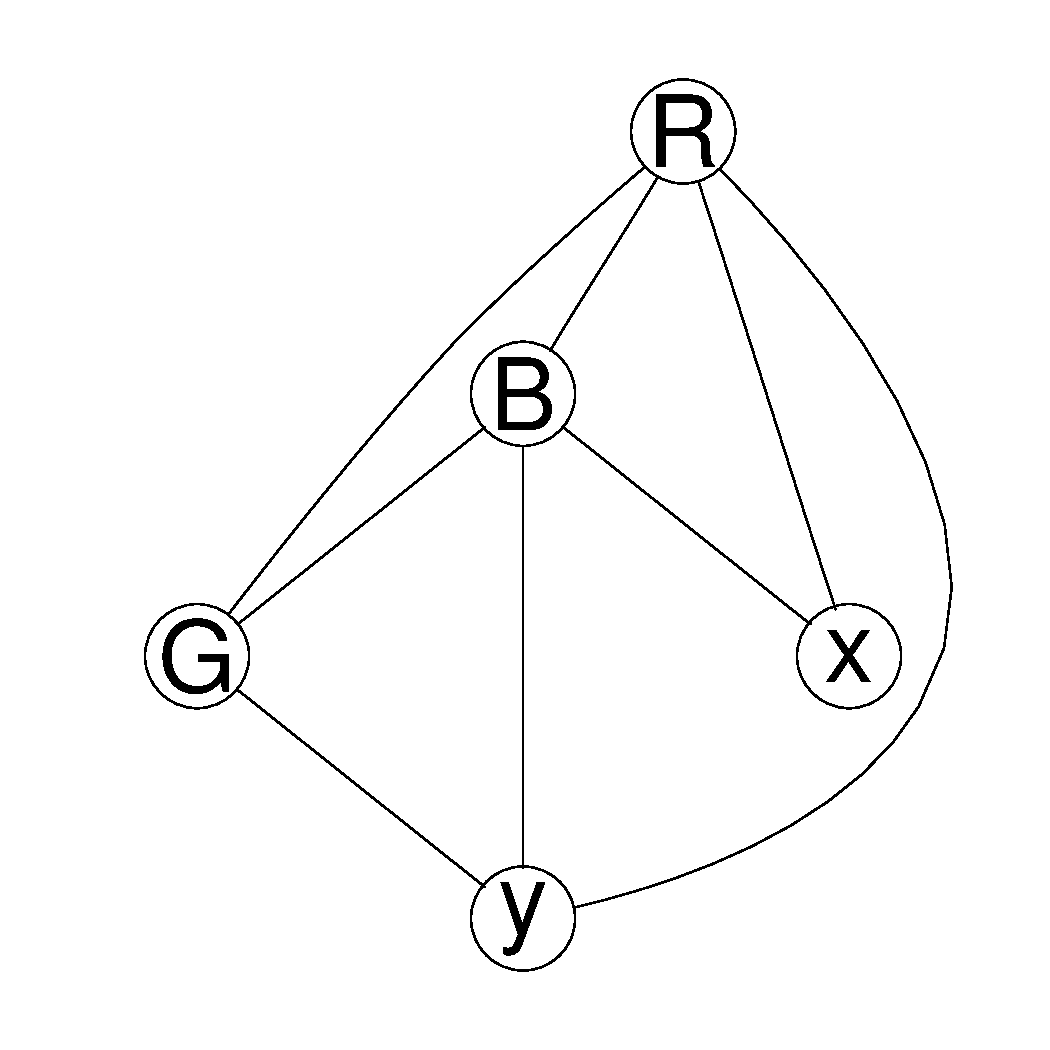
\includegraphics[width=0.6\textwidth]{ggm}
  \caption{Gaussian graphical model determined by backward elimination.}
  \label{fig:ggm}
\end{figure}



\begin{table}[h] \centering 
\begin{tabular}{l|rrrrr} 
R & 0.092  &        &        &       &       \\
G & -0.006 & 0.062  &        &       &       \\
B & -0.071 & -0.007 & 0.085  &       &       \\
x & -0.042 & 0.000  & 0.039  & 0.029 &       \\
y & -0.012 & 0.034  & -0.006 & 0.002 & 0.029 \\
\midrule
  & R      & G      & B      & x     & y     \\ 
\end{tabular} 
\caption{The fitted matrix $V$ based on maximum likelihood estimation using IPF.}
\label{tab:V}
\end{table} 


The sample variance matrix $S$ can be seen in Section~\ref{sec:llsp}.
This leads to the matrix in Table~\ref{tab:V}. Due to the indepence
statements, the values $\hat{v}_{xy}$ and $\hat{v}_{Gx}$ (and their
adjoints) change.

%\subsubsection{Inference}

%In a first step, the covariance matrix and its inverse are
%computed. Then the partial correlations are obtained.

% Construct graph, test for goodness of fit

\subsection{Vine Copula}
The parameters of the fitted vine copula can be seen in
Table~\ref{tab:vine}.

\begin{table}[h]
  \centering
  \footnotesize
  \begin{tabular}{rrlrrrr}
    \toprule
    tree & edge      & family                          & par          & par2         & tau   \\
    \midrule
    1    & 4,3       & Frank                           & 10.52 (0.49) & -            & 0.68  \\
         & 1,4       & Frank                           & -9.46 (0.47) & -            & -0.65 \\
         & 5,1       & Rotated Tawn type 2 270 degrees & -3.02 (0.30) & 0.28 (0.02)  & -0.24 \\
         & 5,2       & Frank                           & 12.01 (0.57) & -            & 0.71  \\
    2    & 1,3;4     & Rotated Tawn type 2 90 degrees  & -2.25 (0.24) & 0.18 (0.03)  & -0.15 \\
         & 5,4;1     & Rotated BB8 90 degrees          & -3.20 (1.08) & -0.72 (0.17) & -0.31 \\
         & 2,1;5     & Rotated Tawn type 1 180 degrees & 2.22 (0.23)  & 0.24 (0.03)  & 0.18  \\
    3    & 5,3;1,4   & Rotated Tawn type 1 270 degrees & -2.09 (0.14) & 0.39 (0.04)  & -0.26 \\
         & 2,4;5,1   & Survival Gumbel                 & 1.11 (0.03)  & -            & 0.10  \\
    4    & 2,3;5,1,4 & Independence                    & -            & -            & 0.00  \\
    \bottomrule
  \end{tabular}
  \caption{Results of the fitting process for vine copulas.}
  \label{tab:vine}
\end{table}
\begin{figure}[h]
  \centering
  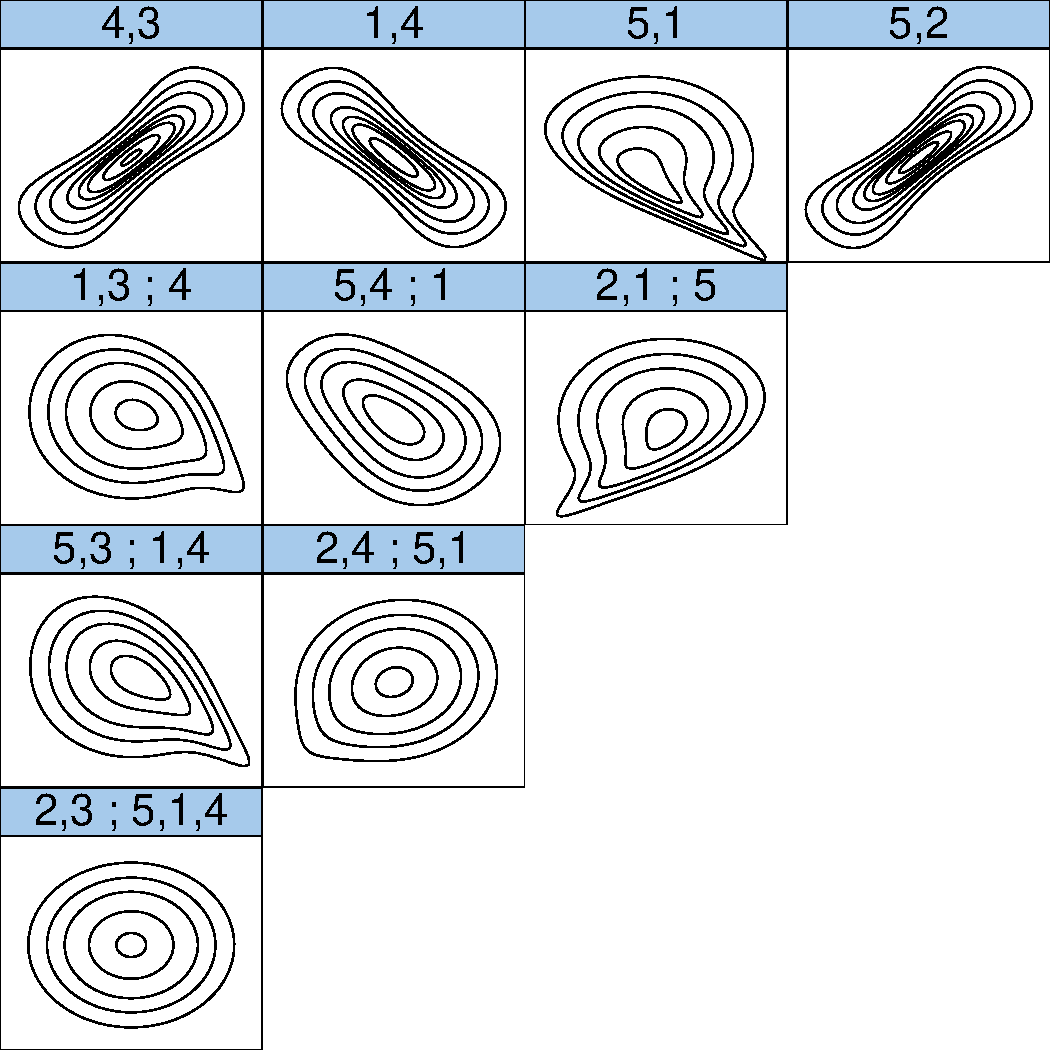
\includegraphics[width=0.6\textwidth]{../algo/R_final/copula_plots/contours}
  \caption{Contour plots with standard normal margins}
  \label{fig:contour}
\end{figure}
Figure~\ref{fig:contour} shows a matrix of
contour plots of the fitted bivariate copula in the vine.  Perpective
visualizations of the density of the used bivariate copulas can be
found in the appendix (\ref{sec:copulas}).
     
\section{Discussion}
\label{sec:discussion}

% TODO: conduct goodness of fit test

This report presented three different approaches for modeling the
dependencies in a five-dimensional regression problem with three
predictors and two target values.\\
Using the linear least squared predictor yielded the highest
RMSE. Using this approach directly, it cannot directly capture
possible independencies in the data, leading to overfitting of the model.\\
The Gaussian graphical model is able to infer independencies leading
to a lower RMSE. The GGM is able to infer the independence between the
random variables $\{G, x\}$ and $\{x, y\}$, leading to more accurate
predictions. The indepencies can be seen in the map image: given all
other variables, the knowledge of $x$ does not contribute to the
knowledge of the green value.

The vine copula shows the best results on the hold-out test set. Since
no clear theory on conditioning vine copulas is existing yet, the mode
of the conditional distribution was calculated by iterating over
possible values. In future research, a more direct approach for
yielding the mode could largely speed-up the process.

% The presented
% results indicate the suitability of our approach.
% While the initially
% chosen image did not allow for modeling the dependency using a
% parametric model, the modification of the map image allowed to
% continue with the analysis.

In future research, several improvements could be made. In a
real-world setting, run-time and computational complexity will be
crucial which we left out here. The used image features consisting of
the mean red, green, and blue value per patch are too simple for
general map images. Therefore, additional features should be included
that are able to describe more sophisticated features, like edges. An
interesting future research direction will be the inclusion of time
dependence: in a real-world scenario, images will not be i.i.d but
highly correlated. This could be modeled using a Bayesian belief
network.


% The presented approach uses simulated data but should be able to
% generalize to real world models.  In a first step, we will select
% suitable features in an iterative approach.


\section{Conclusion}
\label{sec:conclusion}

%In this report, the suitability of independence graphs for computer
%vision-based localization was shown. While the straight-forward
%application of linear regression was not able to capture the structure
%in the generated dataset, a modification of the image underlying the
%data set allowed to generate a simple and effective model, which lead
%to low mean squared errors.

In this report, we compared linear regression, graphical Gaussian
models and vine copulas for the dependence modeling of variables in a
computer vision task. 

\printbibliography
\appendix

%\section{Supplementary Material}

\clearpage
\begin{samepage}
  \section{Visualization of the used copulas}
  \label{sec:copulas}
  \subsection{Tree 1}
  \begin{figure}[h]
    \begin{subfigure}[b]{0.475\textwidth}
      \centering
      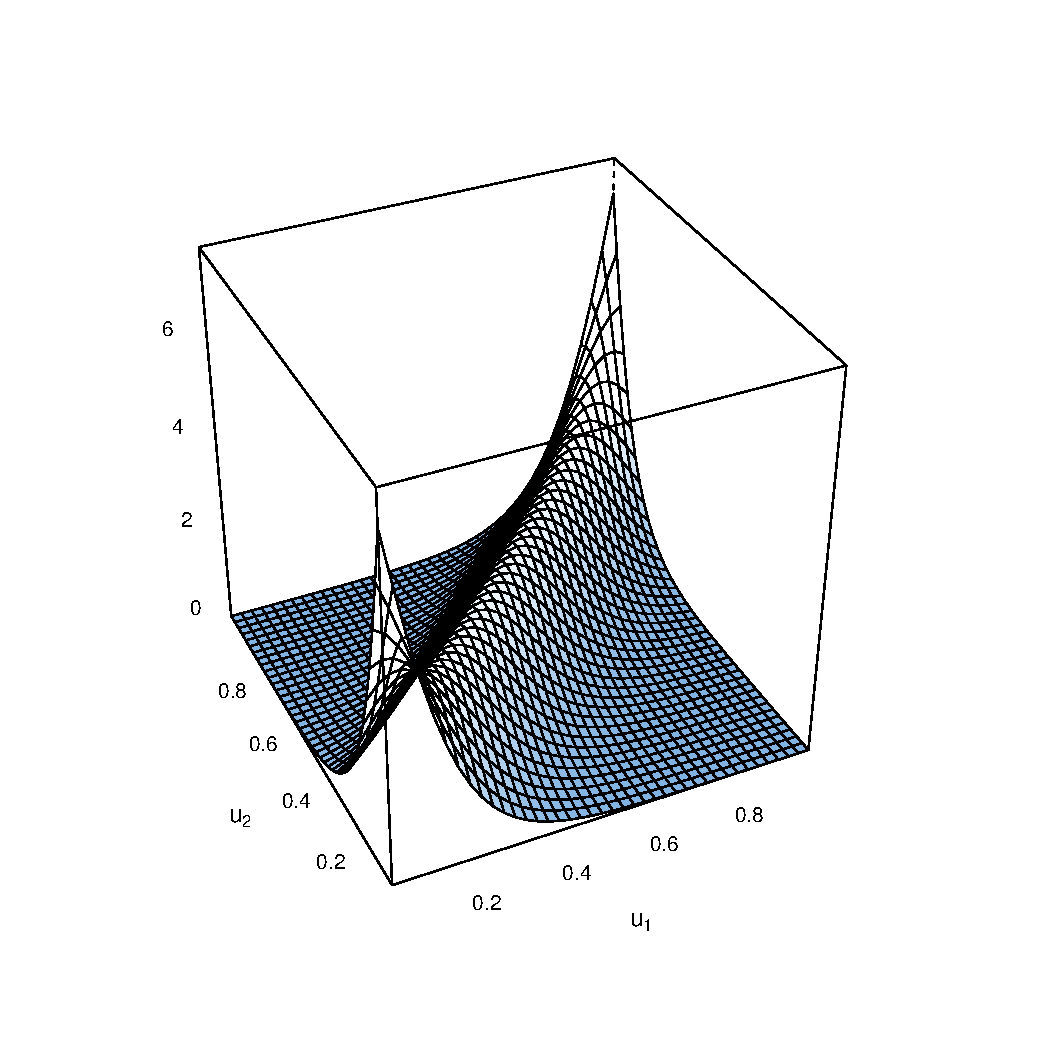
\includegraphics[width=\textwidth]{1}
      \caption[]%
      {{\small 4,3 Frank (par = 10.52, tau = 0.68)}}
      \label{fig:a}
    \end{subfigure}%
    \hfill
    \begin{subfigure}[b]{0.475\textwidth}
      \centering
      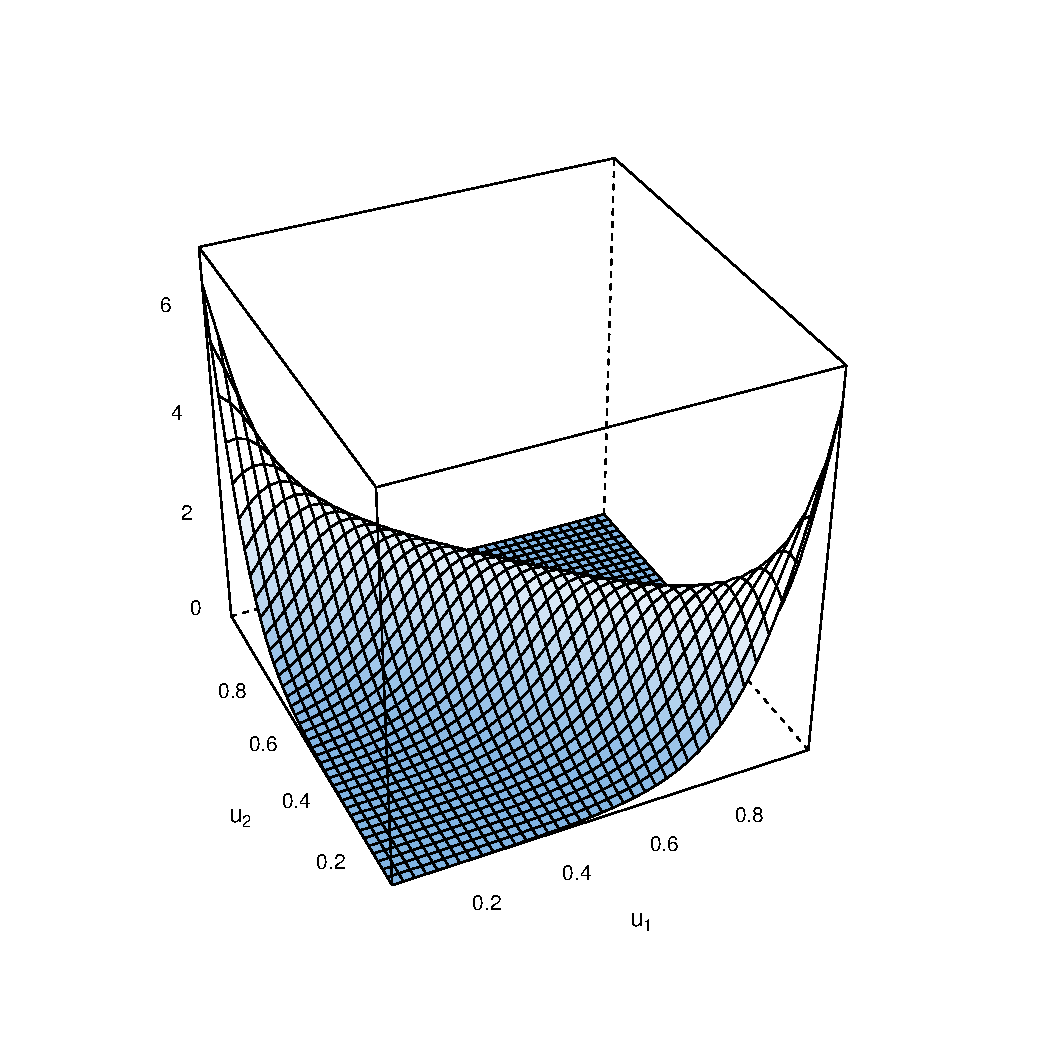
\includegraphics[width=\textwidth]{2}
      \caption[]%
      {{\small 1,4 Frank (par = -9.46, tau = -0.65)}}
      \label{fig:b}
    \end{subfigure}

  \begin{subfigure}[b]{0.475\textwidth}
    \centering
    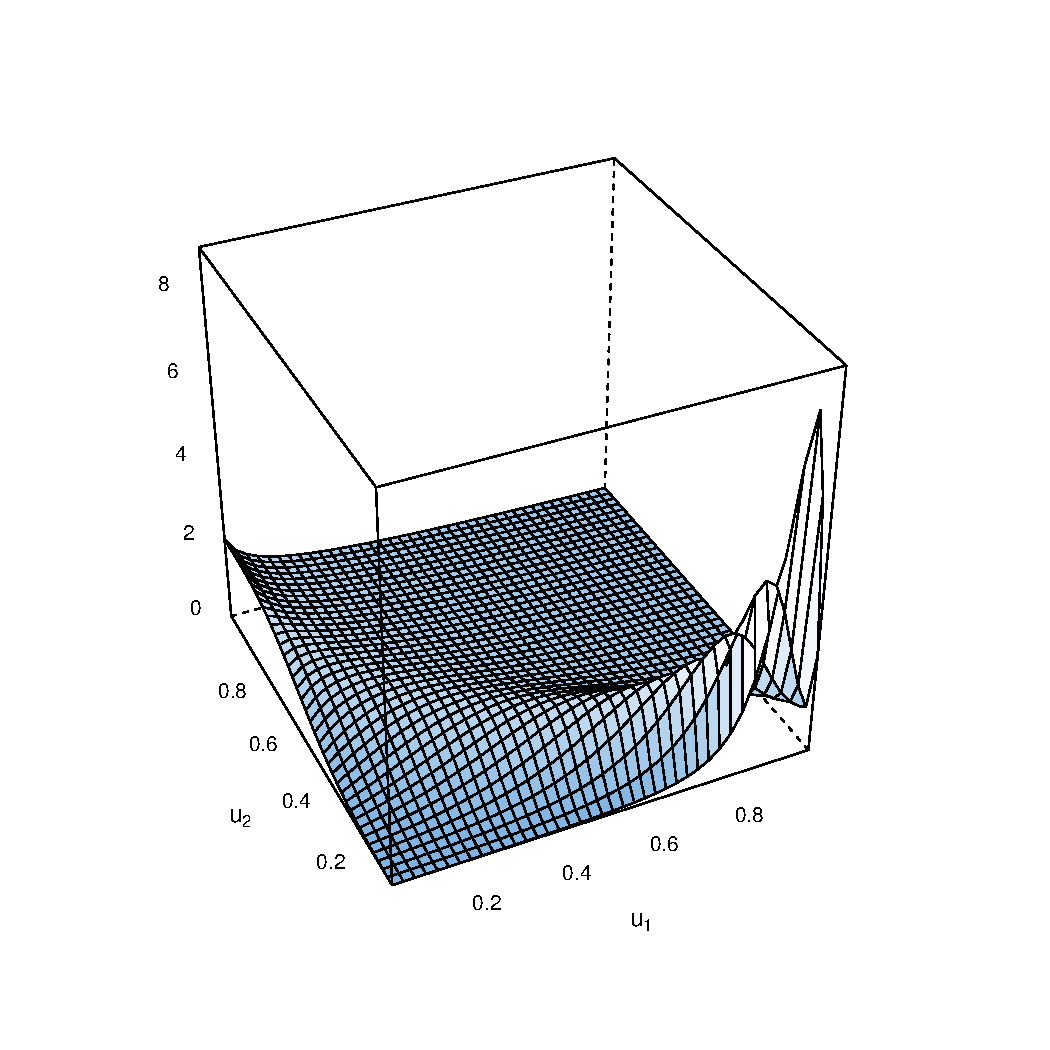
\includegraphics[width=\textwidth]{3}
    \caption[]%
    {{\small 5,1 Rotated Tawn type 2 270 degrees (par = -3.02, par2 =
        0.28, tau = -0.24)}}
    \label{fig:c}
  \end{subfigure}
  \hfill
  \begin{subfigure}[b]{0.475\textwidth}
    \centering
    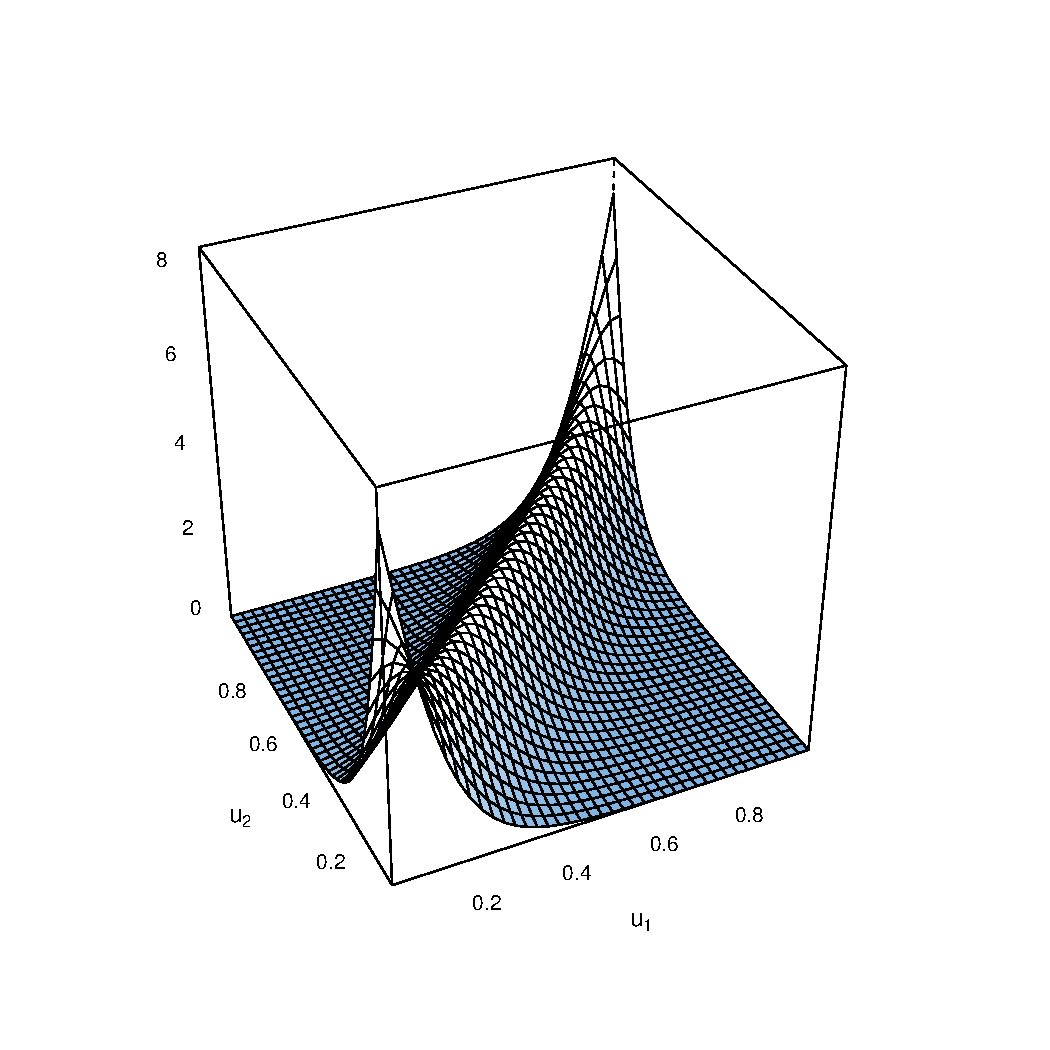
\includegraphics[width=\textwidth]{4}
    \caption[]%
    {{\small 5,2 Frank (par = 12.01, tau = 0.71)}}
    \label{fig:d}
  \end{subfigure}
  \caption[ Global caption ]
  {\small Perspective visualization of the density of the used
    bivariate copulas for tree 1.}
  \label{fig:test-figure}
\end{figure}
\end{samepage}
\clearpage
\section{Dataset with average red, green, and blue values}
\begin{center}
  \csvautotabular{all_vals.csv}
\end{center}

\clearpage
\section{Technical Report}
\label{sec:technical}

The code for generating the graphs and yielding the results presented
in this report was written in \texttt{R}. The used data is saved in
CSV format. Both can be found on GitHub:\\
\noindent\url{https://github.com/Pold87/decision-theory}\\

% The section for the linear regression made use of th

The section on Graphical Gaussian Models made use of the packages
\texttt{gRim, gRbase} and \texttt{Rgraphviz} for the visualization.\\

The section on VineCopula used the packages \texttt{copula} and
\texttt{VineCopula}.

\end{document}
